% Chapter 3

\chapter{Development of Artefact and Article} % Main chapter title

\label{Chapter3} % For referencing the chapter elsewhere, use \ref{Chapter3} 

This chapter describes the artefact that was developed in a group effort as well as the process followed for the writing of the academic article.

\section{Description of Artefact and Article}
This research project was split into two main aspects: 
\begin{enumerate}
\item An individual research study into a chosen topic \textit{(this being the qualities needed for a computer game to be used in education)}
\item A group effort to develop a digital computer game.
\end{enumerate}

\noindent For the first aspect of this project, the resulting outcome was an academic article titled, \textit{"Linking Gamification, Ludology and Pedagogy: How to Use Serious Games for Various Knowledge Domains"}. As stipulated in the title, the fields of gamification, ludology and pedagogy were the focus of this research aspect of the project. In this article, the question posed by this project is again reiterated and sequentially answered. The article is attached to this document under Appendix  \ref{AppendixC}. 
\\\\
The artefact accompanying this research project is a digital computer came which was developed as part of a group effort as mentioned previously. While this artefact is separate from the individual research studies conducted by its' group members, it may have been influenced by the topics being researched. The artefact is titled \textit{"Puzzle Ball: Spherical Shadows"} and is further categorised as a 3D puzzle platformer with aspects of action gameplay played in first person. A playable version of the artefact is available on the website itch.io website\footnote{\url{https://josh-scg.itch.io/puzzle-ball-spherical-shadows}} and the source code of the artefact is available on GitHub\footnote{\url{https://github.com/GCWehmeyer/Spherical_Shadows}}$^{,}$\footnote{\url{https://github.com/Josh-SCG/Spherical_Shadows}}

\section{Artefact Life Cycle Followed and its Different Phases}
% Briefly provide general background on the life cycle that was followed and why it is appropriate to this artefact.

\section{Description of the Development of the Artefact}
%Comprehensive report on the way in which each phase of the life cycle was applied in the development of this artefact.


%Full Level
\begin{figure}[H]
\centering
\begin{subfigure}{0.5\textwidth}
  \centering
  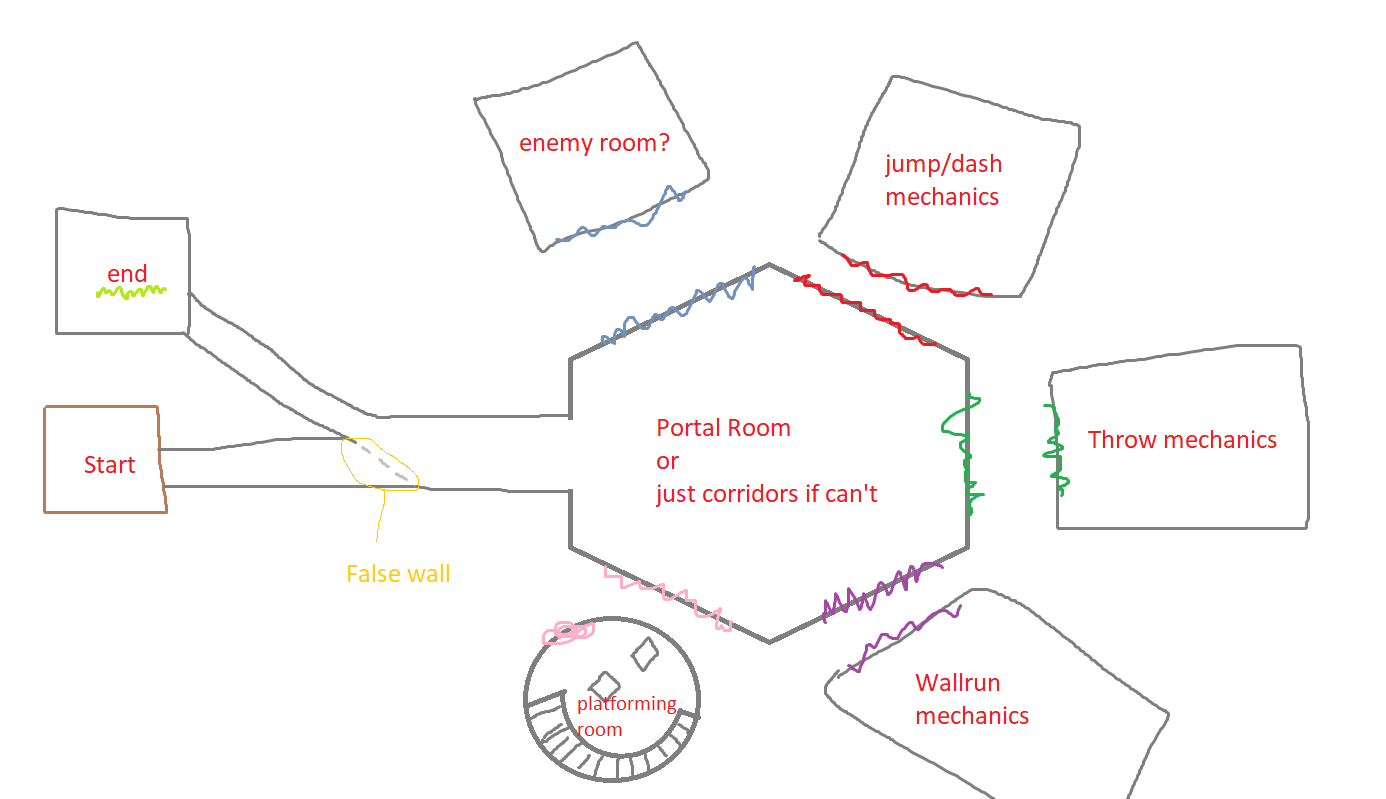
\includegraphics[width=1\linewidth]{Figures/fullplan.png}
  \caption{Provisional Plan}
\end{subfigure}%
\begin{subfigure}{0.5\textwidth}
  \centering
  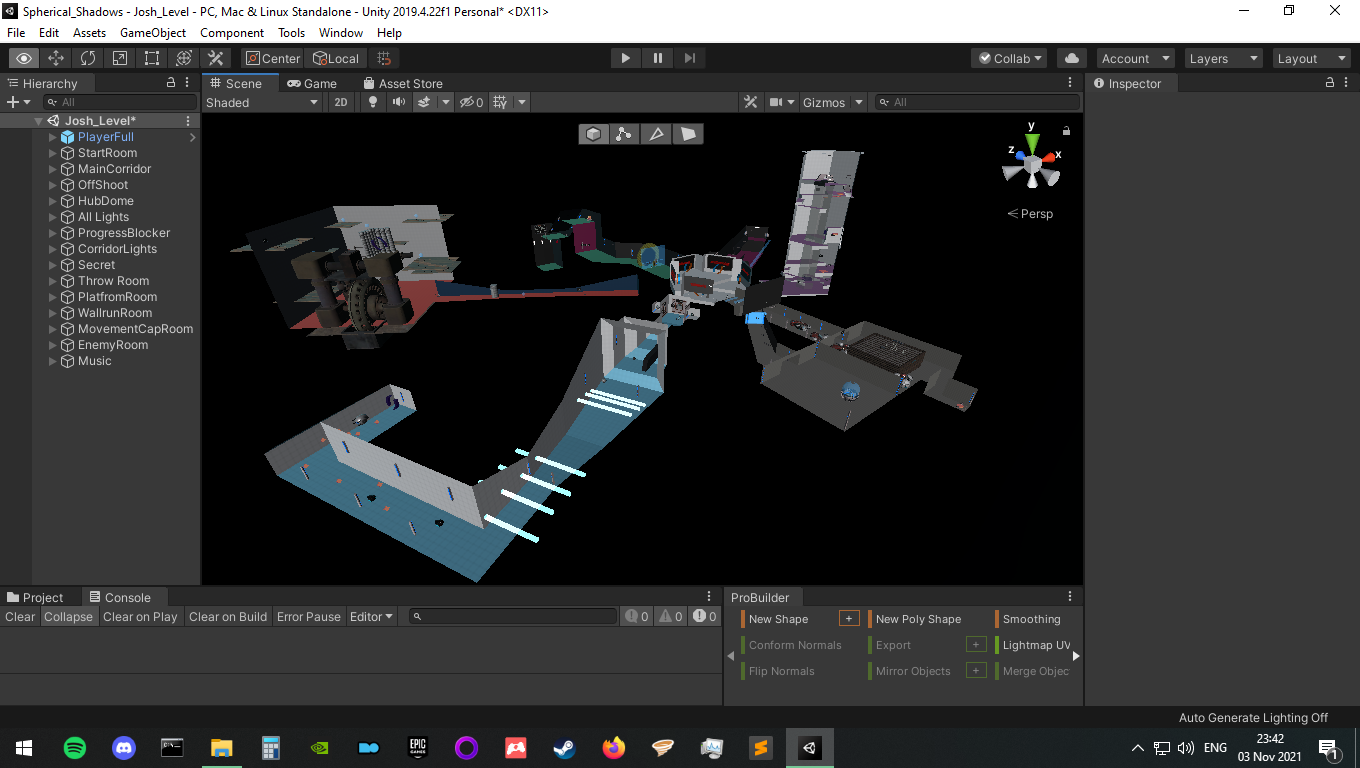
\includegraphics[width=1\linewidth]{Figures/full.png}
  \caption{Screenshot in Unity Editor}
\end{subfigure}
\caption{Layout of Full Level (Tutorial)}
\end{figure}


%Hub
\begin{figure}[H]
\centering
\begin{subfigure}{0.5\textwidth}
  \centering
  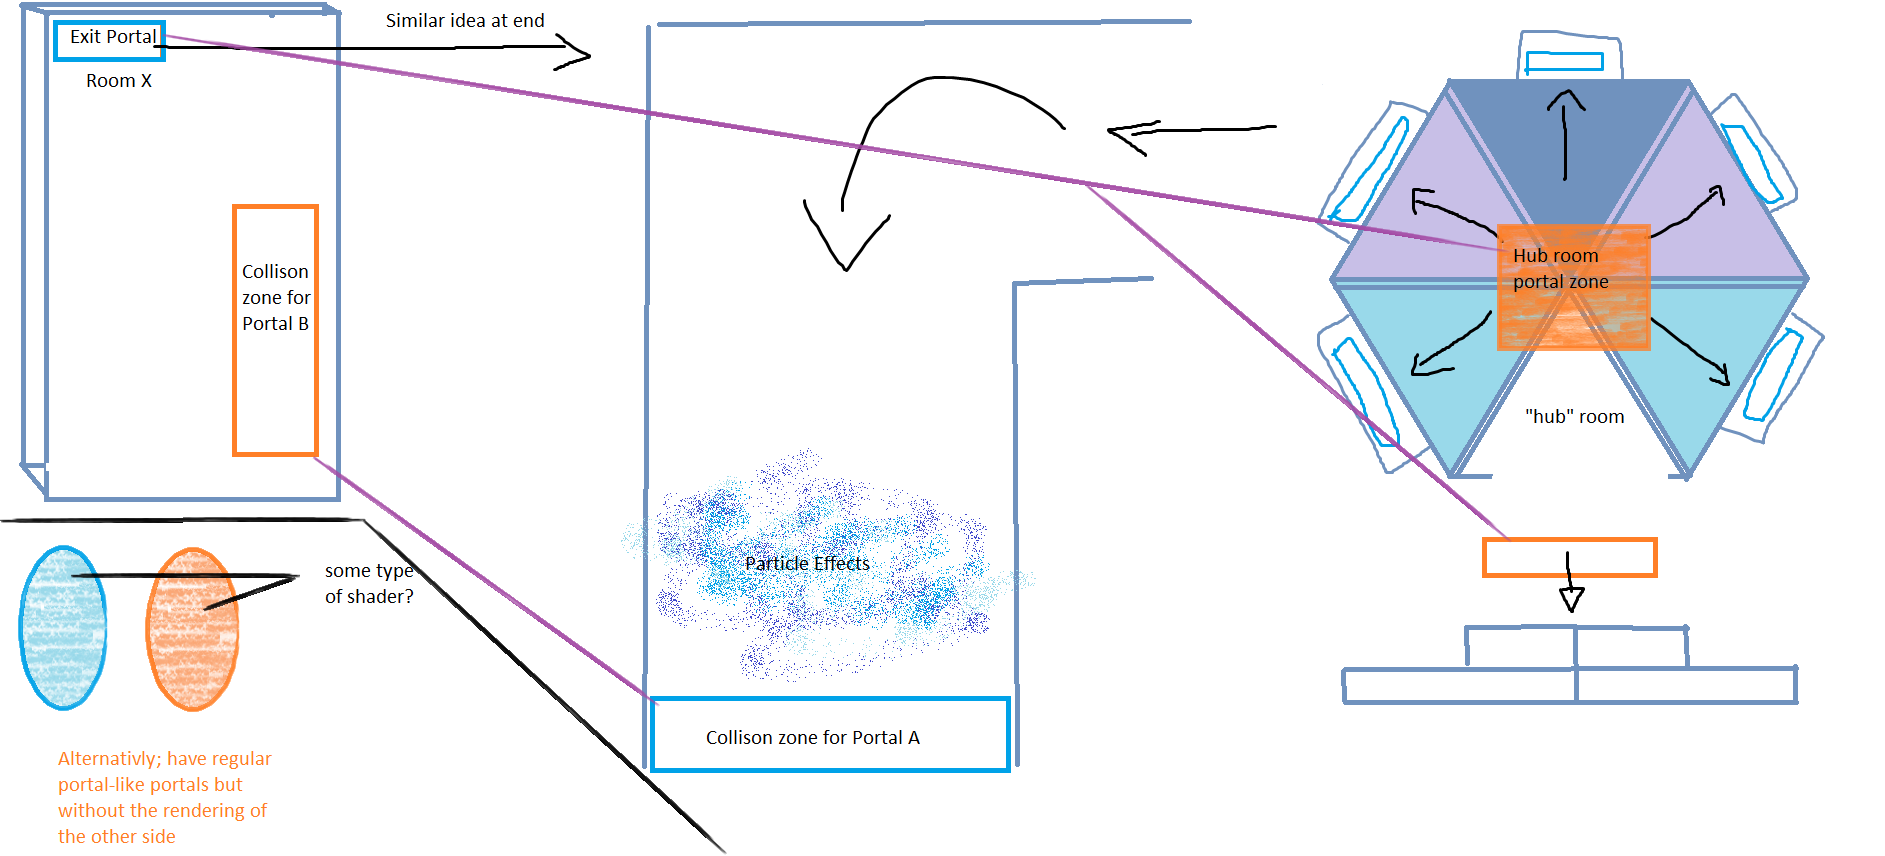
\includegraphics[width=1\linewidth]{Figures/hubplan.png}
  \caption{Provisional Plan}
\end{subfigure}%
\begin{subfigure}{0.5\textwidth}
  \centering
  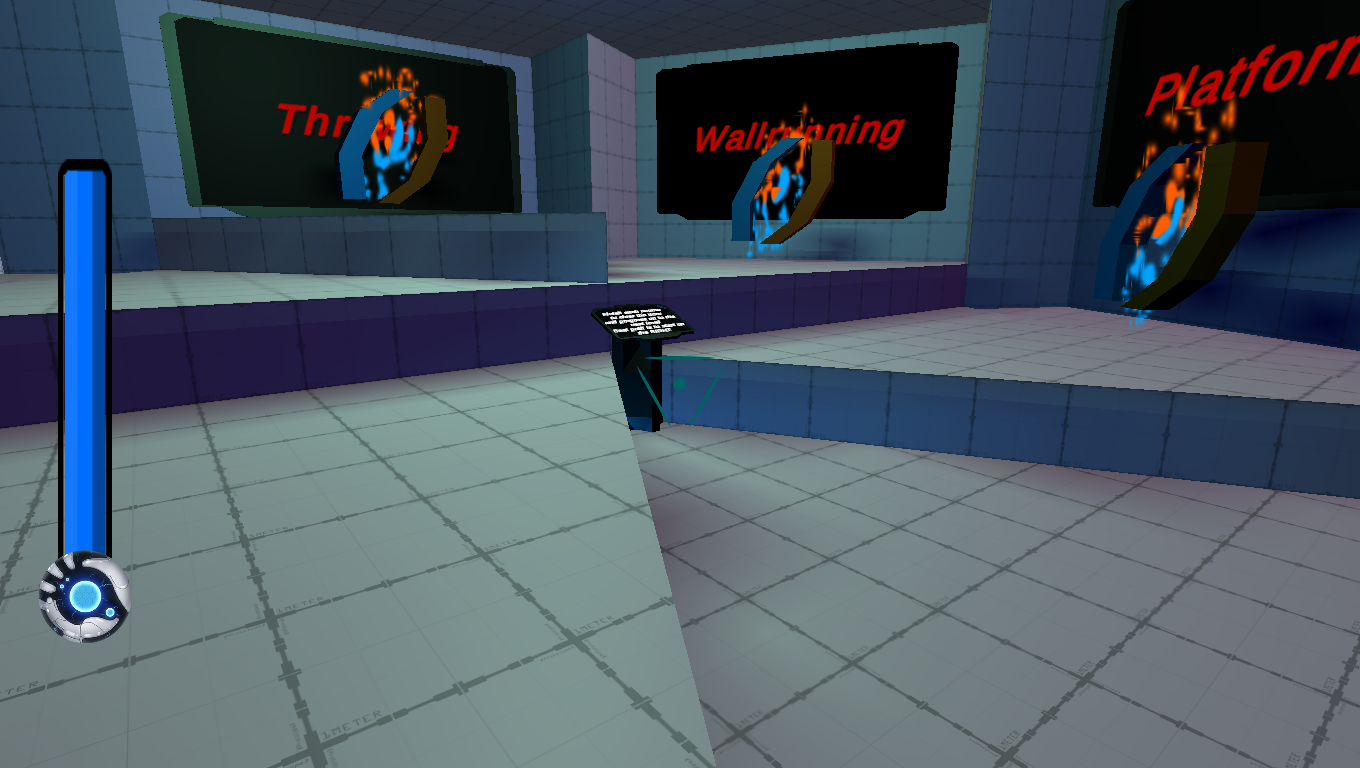
\includegraphics[width=1\linewidth]{Figures/hub.png}
  \caption{Screenshot in Artefact}
\end{subfigure}
\caption{Layout of Hub Room}
\end{figure}


%Platform
\begin{figure}[H]
\centering
\begin{subfigure}{0.5\textwidth}
  \centering
  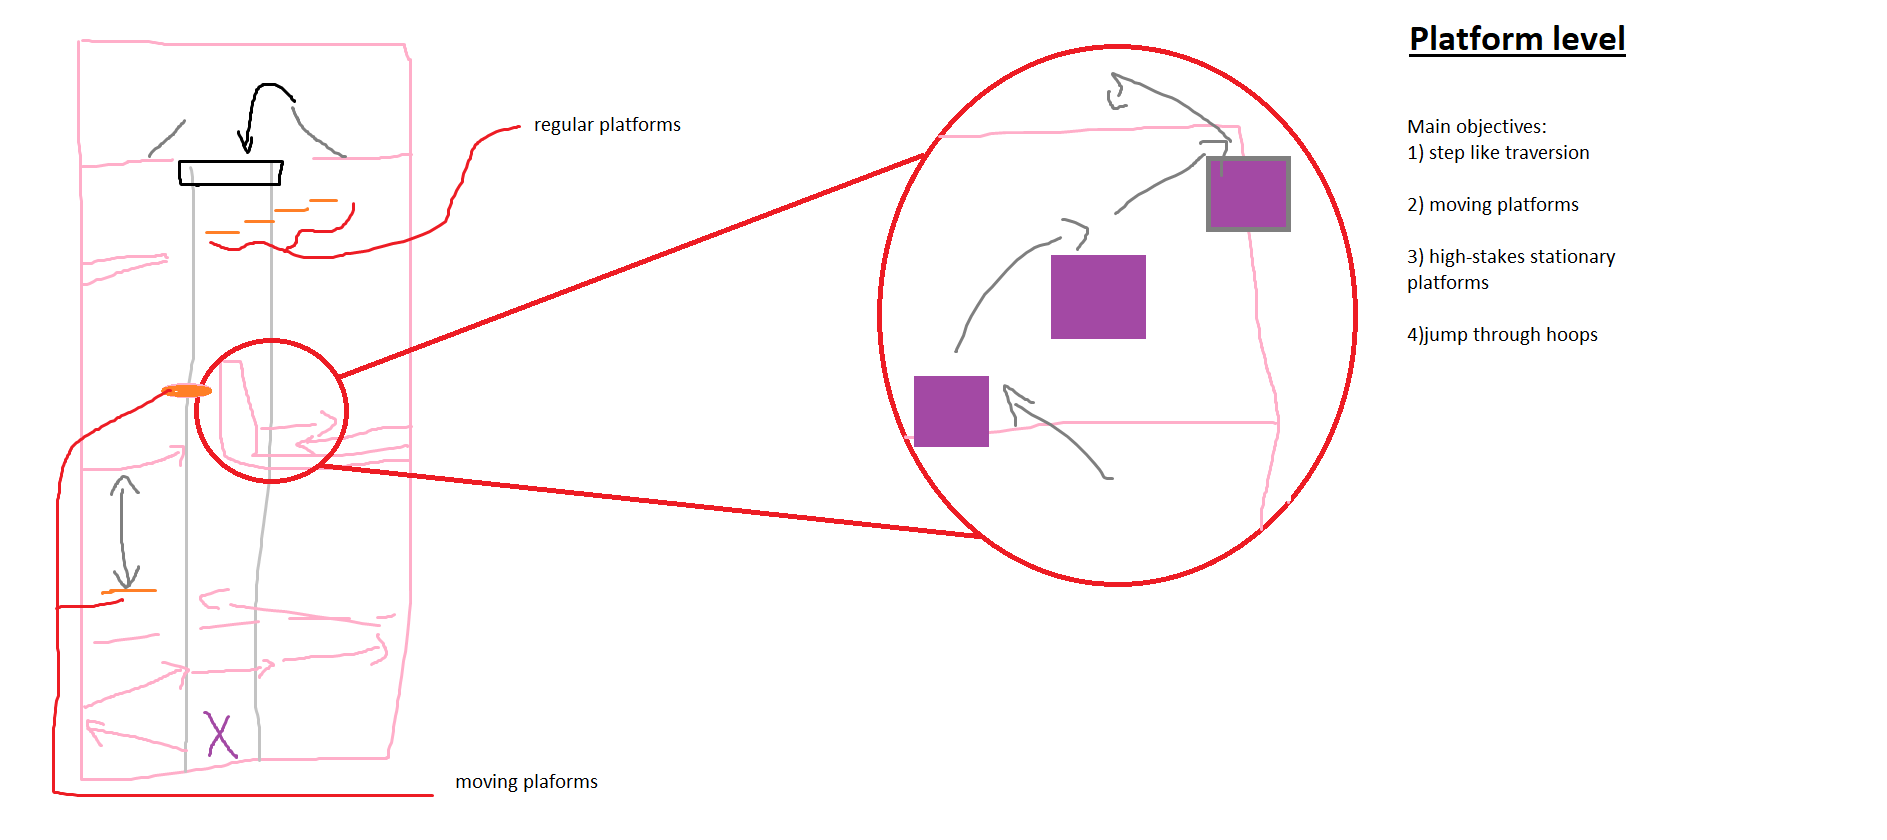
\includegraphics[width=1\linewidth]{Figures/platformplan.png}
  \caption{Provisional Plan}
\end{subfigure}%
\begin{subfigure}{0.5\textwidth}
  \centering
  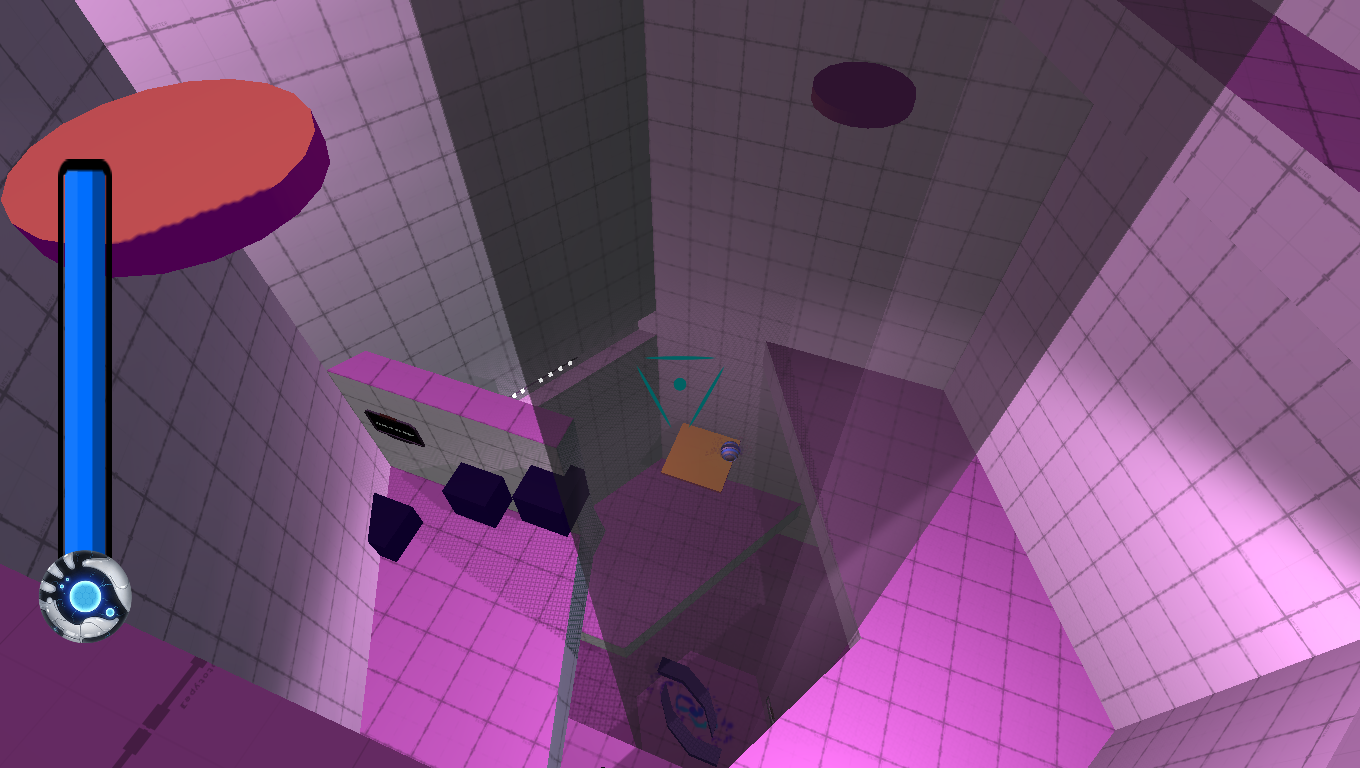
\includegraphics[width=1\linewidth]{Figures/platform.png}
  \caption{Screenshot in Artefact}
\end{subfigure}
\caption{Layout of Platforming Tutorial}
\end{figure}

%WallRun
\begin{figure}[H]
\centering
\begin{subfigure}{0.5\textwidth}
  \centering
  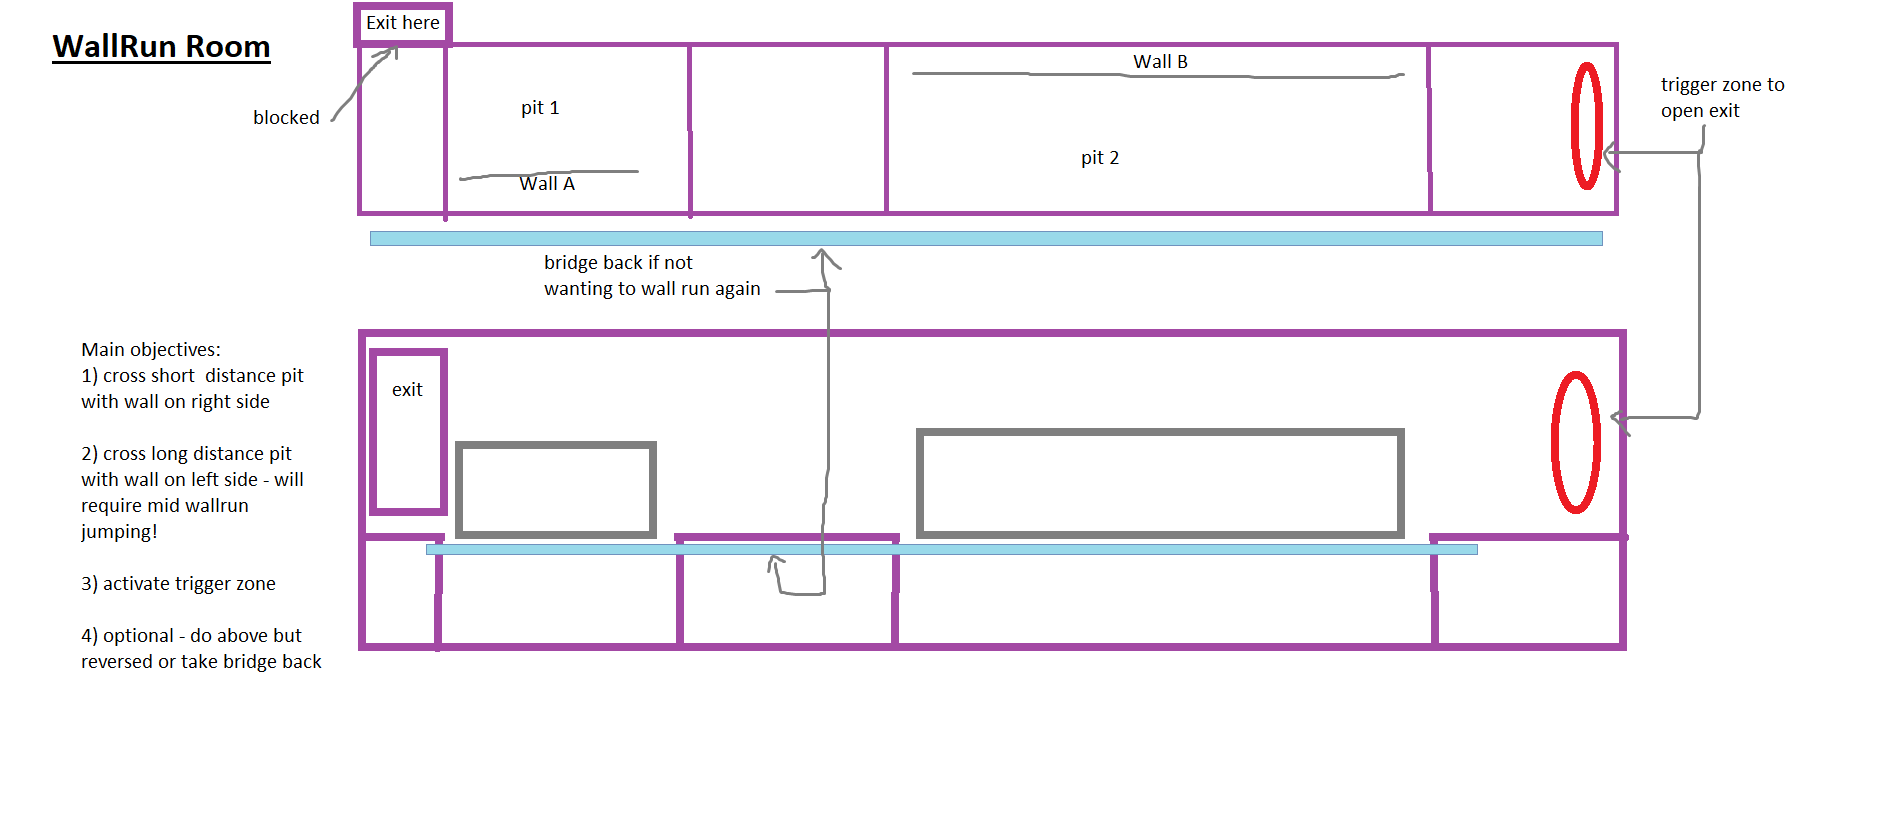
\includegraphics[width=1\linewidth]{Figures/wallplan.png}
  \caption{Provisional Plan}
\end{subfigure}%
\begin{subfigure}{0.5\textwidth}
  \centering
  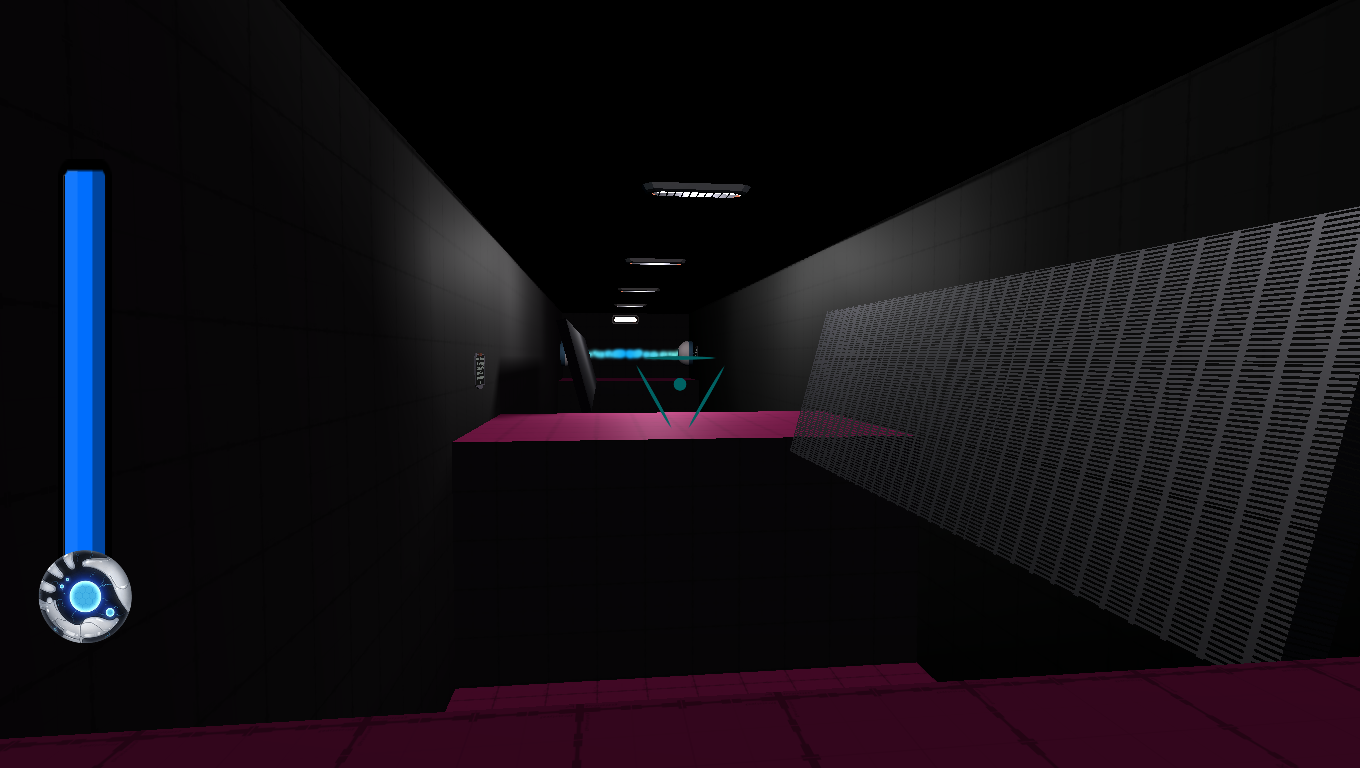
\includegraphics[width=1\linewidth]{Figures/wall.png}
  \caption{Screenshot in Artefact}
\end{subfigure}
\caption{Layout of Wall Running Tutorial}
\end{figure}

%Throw
\begin{figure}[H]
\centering
\begin{subfigure}{0.5\textwidth}
  \centering
  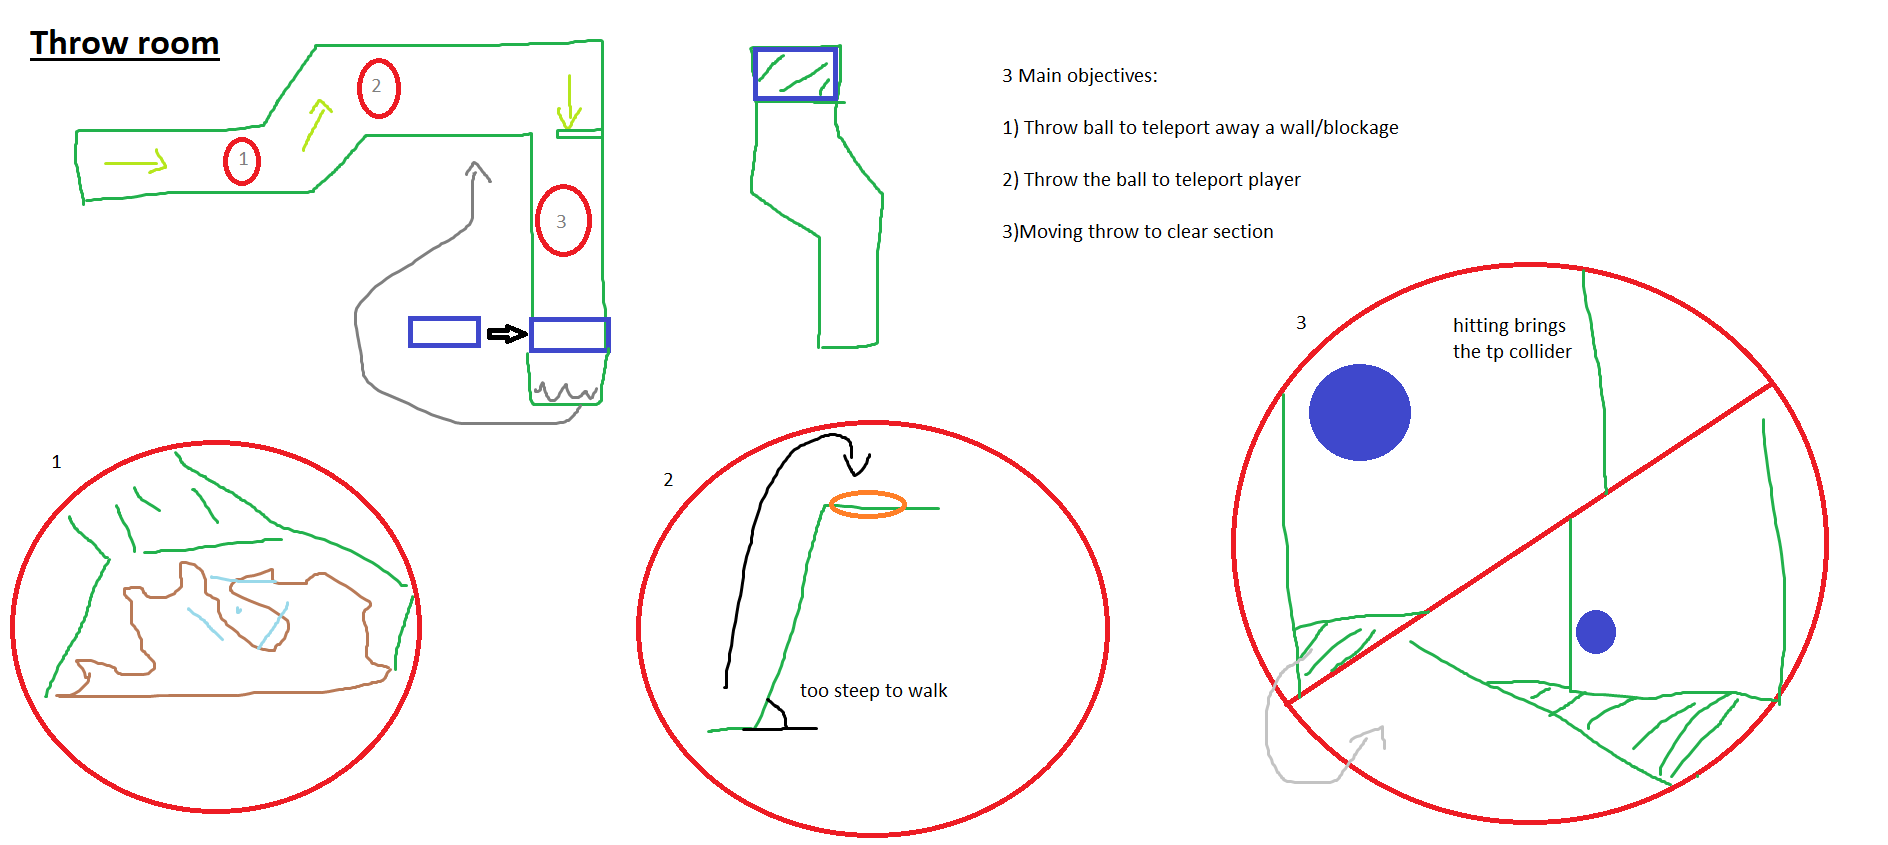
\includegraphics[width=1\linewidth]{Figures/throwplan.png}
  \caption{Provisional Plan}
\end{subfigure}%
\begin{subfigure}{0.5\textwidth}
  \centering
  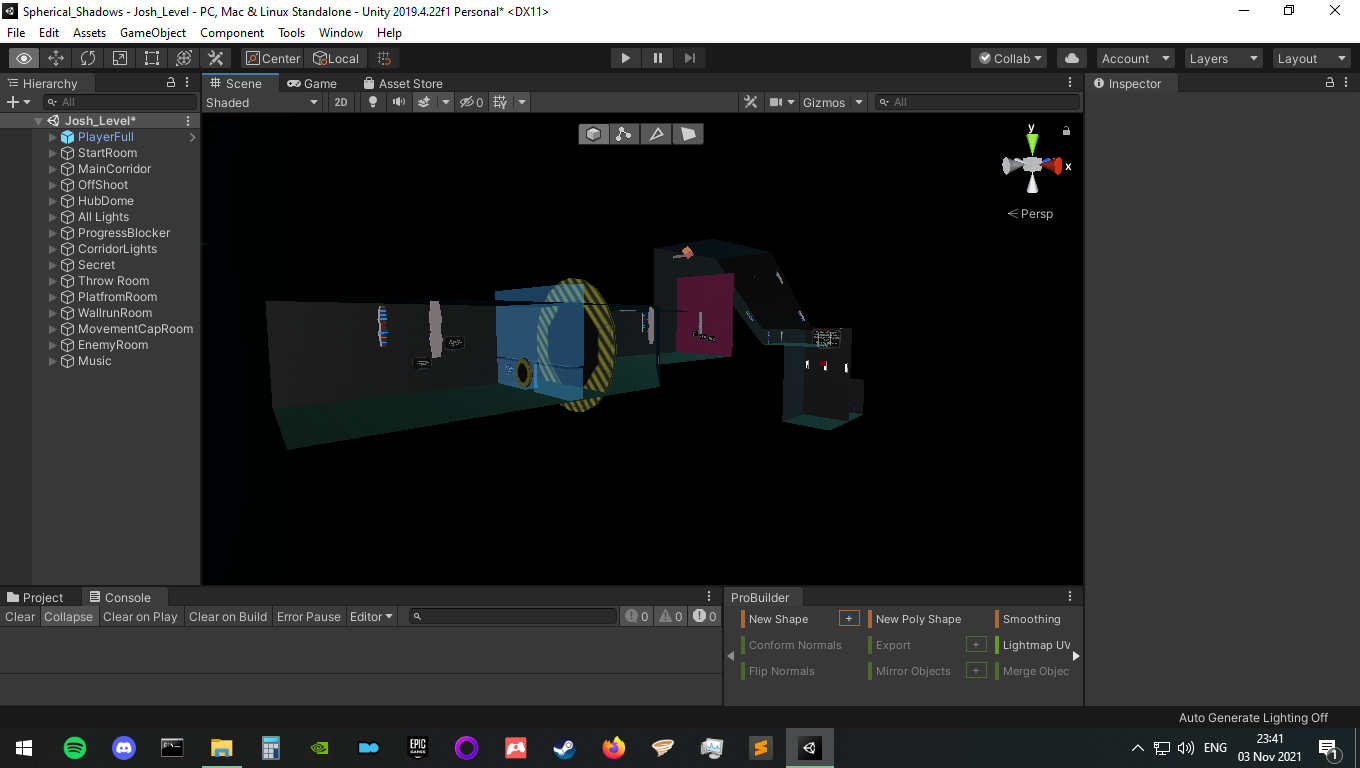
\includegraphics[width=1\linewidth]{Figures/throw.png}
  \caption{Screenshot in Unity Editor}
\end{subfigure}
\caption{Layout of Throw Tutorial}
\end{figure}


%Mcap
\begin{figure}[H]
\centering
\begin{subfigure}{0.5\textwidth}
  \centering
  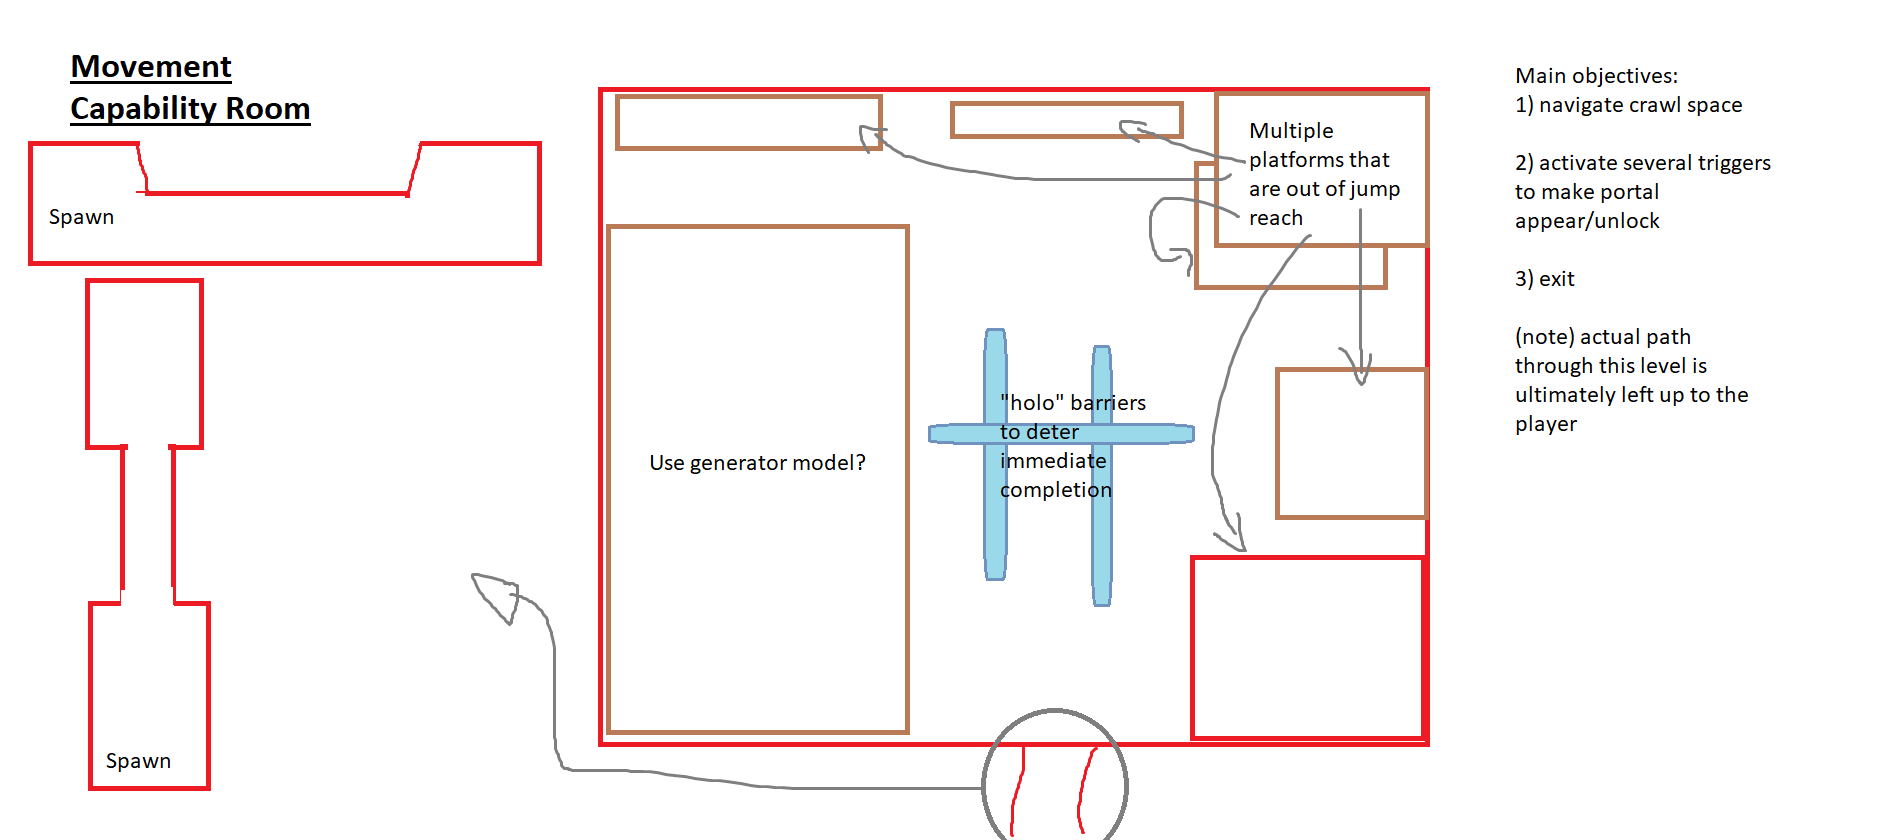
\includegraphics[width=1\linewidth]{Figures/mcapplan.png}
  \caption{Provisional Plan}
\end{subfigure}%
\begin{subfigure}{0.5\textwidth}
  \centering
  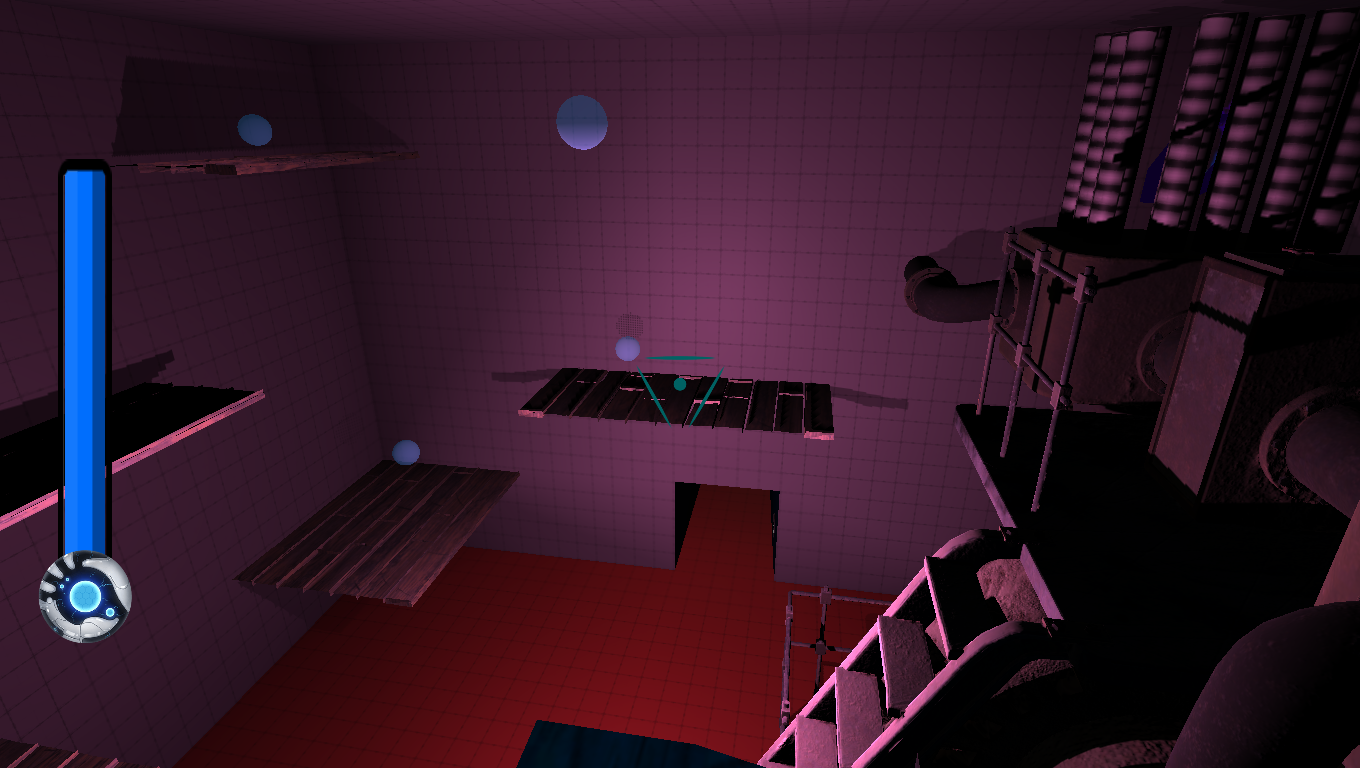
\includegraphics[width=1\linewidth]{Figures/mcap.png}
  \caption{Screenshot in Artefact}
\end{subfigure}
\caption{Layout of Movement Tutorial}
\end{figure}

%Enemy
\begin{figure}[H]
\centering
\begin{subfigure}{0.5\textwidth}
  \centering
  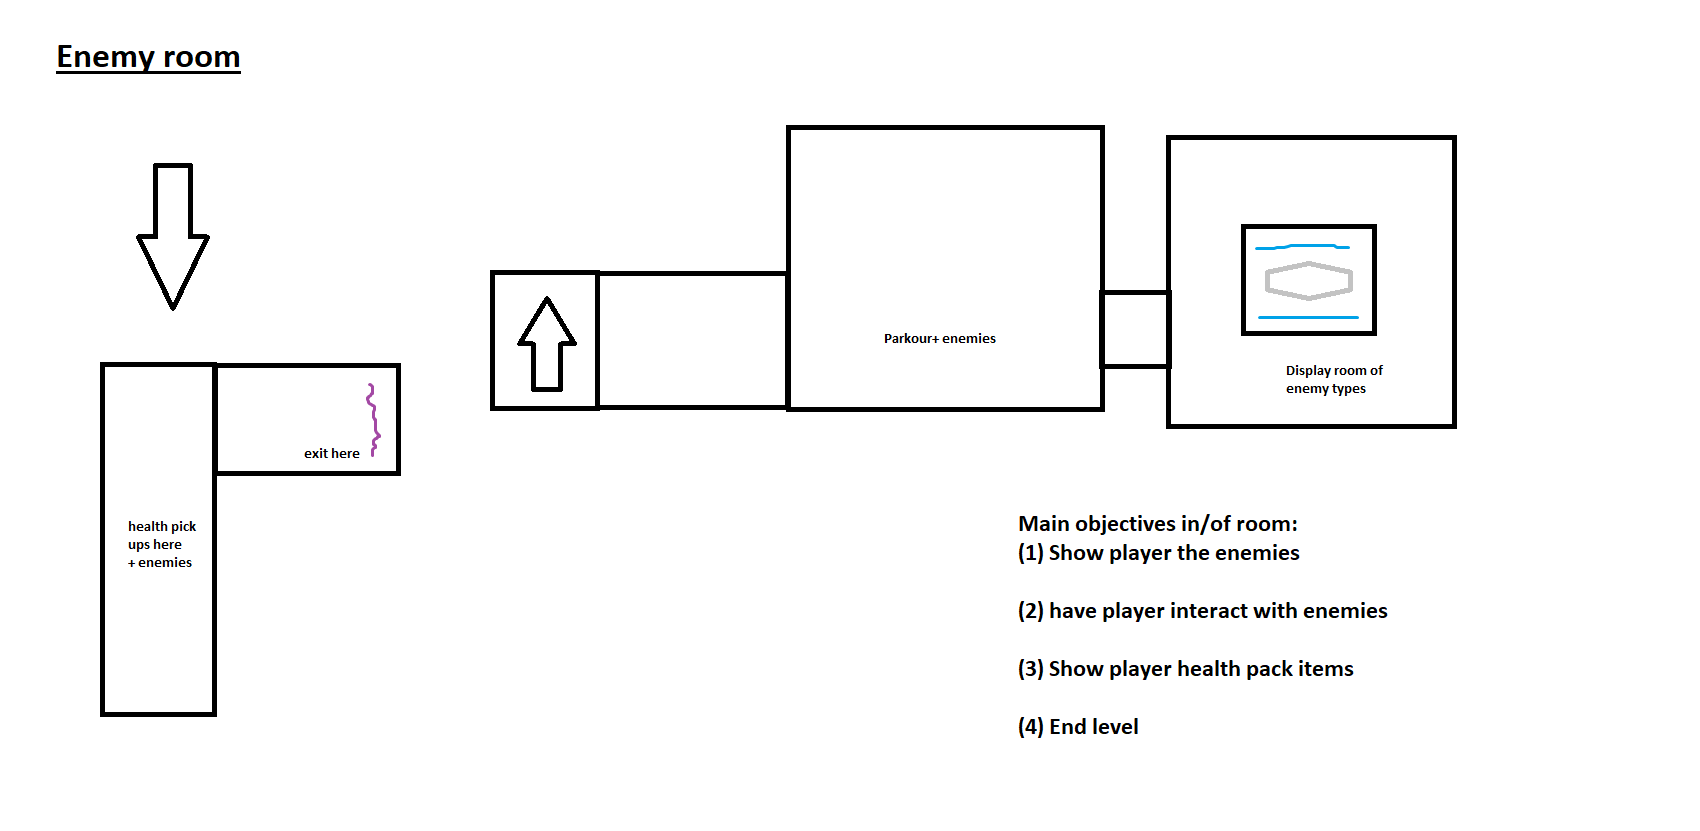
\includegraphics[width=1\linewidth]{Figures/enemyplan.png}
  \caption{Provisional Plan}
\end{subfigure}%
\begin{subfigure}{0.5\textwidth}
  \centering
  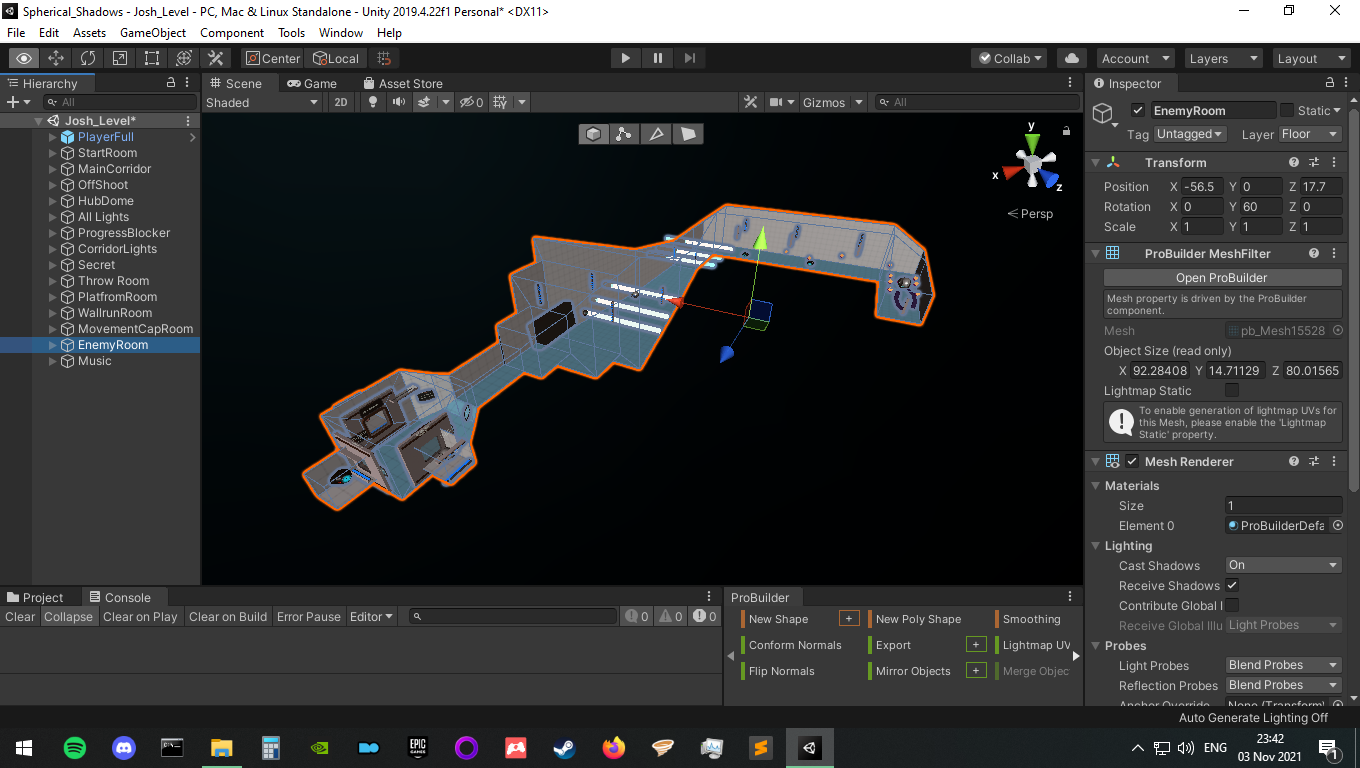
\includegraphics[width=1\linewidth]{Figures/enemy.png}
  \caption{Screenshot in Unity Editor}
\end{subfigure}
\caption{Layout of Enemy Tutorial}
\end{figure}

\section{Conclusion}